\chapter{Preprocessing}
\label{ch:preprocessing}
Before testing and assessing source separation algorithms, the raw EMG recordings must be transformed to facilitate the signal analysis. This preprocessing stage is especially important in this work because the objective is not only to visualize or classify EMG activity, but to separate weak target components from stronger interfering muscular sources. Therefore, small differences in amplitude, noise level or signal spectral structure can strongly affect the behavior of ICA, SOBI and the constrained separation methods considered later on this work.

As mentioned in section \ref{subsec:tmr_dataset}, the dataset used in this study is 32 channel surface EMG. This chapter will mention the preprocessing for the TMR dataset, but it may also be applied to 2 channel invasive measurements, like in the IIT study.

The preprocessing pipeline developed in this work includes three main stages. First, the observed signals are filtered to eliminate any artifacts or interferences that contaminate the EMG signal during the recording. After this, each channel is scaled to fairly compare different muscle signals. Finally, the observations are whitened to decorrelate the signals and facilitate the separation process. Figure \ref{fig:preprocessing_pipeline} shows a conceptual diagram to better understand this pipeline.

\begin{figure}[H]
    \centering
    \makebox[\textwidth][c]{%
        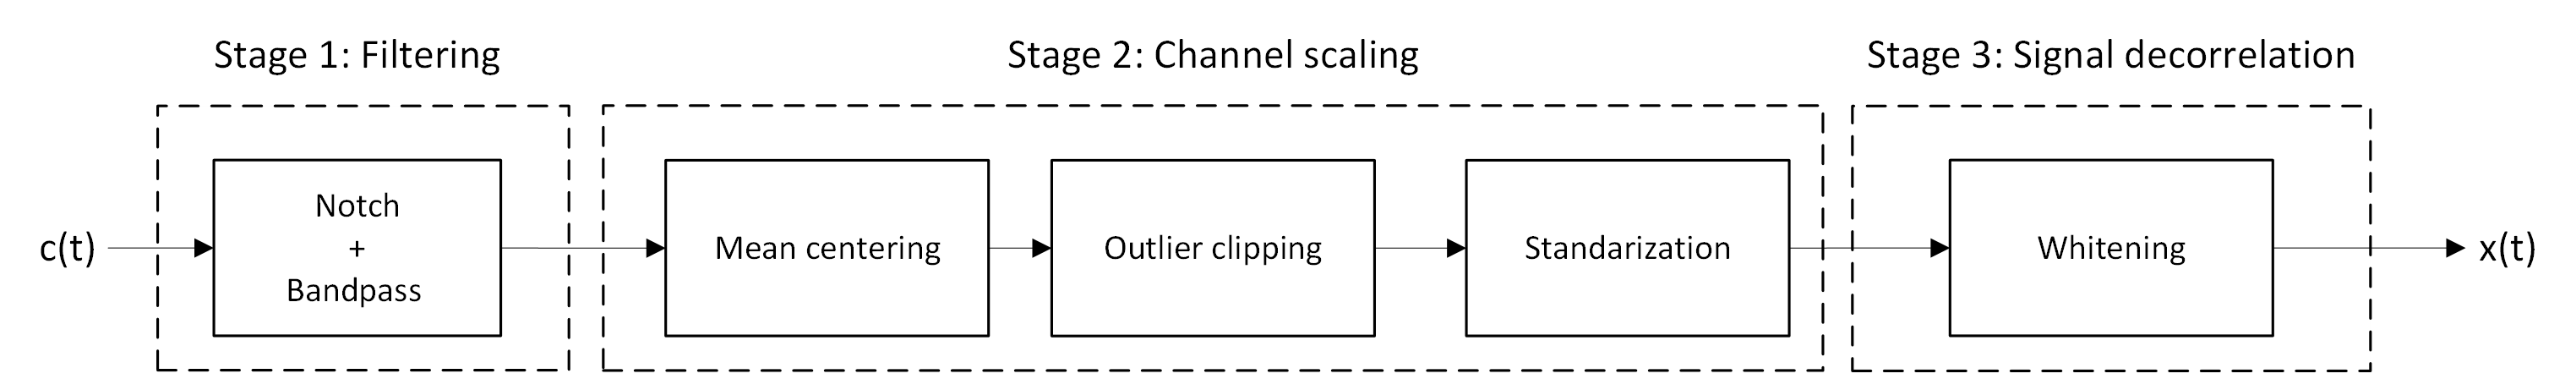
\includegraphics[width=1.25\linewidth]{figuras/preprocessing/preprop_diagram.png}%
    }
    \caption{Preprocessing pipeline applied to the observed EMG mixtures $c(t)$ to transform data into valid inputs $x(t)$ for the separation algorithms. The pipeline is divided into three stages: filtering, channel scaling and signal decorrelation.}
    \label{fig:preprocessing_pipeline}
\end{figure}

\section{Filtering}

Raw EMG recordings may often contain undesired components introduced by noise, movement artifacts, baseline drift and other possible sources of interferences. For this reason, the first step in the preprocessing pipeline must be reduce these unwanted components. Separation algorithms rely on series of assumptions, such as covariance and autocorrelation of the signals, that would not hold without reducing these components. 

Additionally, since we are also contemplating a possible live implementation, the selected approach prioritizes a low-complexity \textbf{causal filter with reduced delay} while also still providing sufficient attenuation outside the selected EMG band. 

\subsection{Filter design}
In order to design the filter, a desired EMG band must be identified first. Generally, the relevant EMG content is considered to lie approximately within the \qtyrange{20}{450}{\hertz} range \cite{powar_novel_2018}. Additionally, in many real live situations, there is a power line interference at \qty{50}{\hertz} or \qty{60}{\hertz}, which pollutes the EMG passband. Given the causality and low delay requirements, the best approach is to mainly consider low order IIR filters. Even though higher order filters would provide steeper transitions, they increase the phase distortion and group delay, which directly affect the real-time analysis of the EMG signals. For simplification, this study mainly considers \textbf{Butterworth} filter design, since its smooth and flat passband response helps preserve the relevant EMG components without passband ripple. Alternatively, a Bessel filter would better preserve the waveform, but this is less critical for the present analysis and Butterworth provides a sharper transition band.

Consequently, this first preprocessing stage must design two filters to address these two specific aspects: a power-line removal filter and a EMG frequency range filter.

\subsubsection{Power-line removal filter}

This filter intends to specifically remove the artifact associated with the power line interference. Since the dataset was collected in the United States, this interference is expected to be located around \qty{60}{\hertz}. For Notch specific characteristics, it is necessary to determine a reasonable stopband to ensure that the power-line interference is minimized. A common Notch bandwidth estimation is the one showed in Equation \ref{eq:notch_bw_calculation}, where $Q$ is the quality factor and $f_{remove}$ is the notch center frequency. Once the bandwidth is obtained, the lower and upper cutoff frequencies can be defined by assuming symmetric rejection band around $f_{remove}$\cite{noauthor_designnotchpeakiir_nodate}.

\begin{equation}
    BW= \frac{f_{remove}}{Q}, \quad f_1=f_{remove}-\frac{BW}{2}, \quad f_2=f_{remove}+\frac{BW}{2}
    \label{eq:notch_bw_calculation}
\end{equation}
In this work, $f_{remove}=\qty{60}{\hertz}$ and $Q=30$ were selected, resulting in a bandwidth of $BW=\qty{2}{\hertz}$. Consequently, the used for the notch filter are $f_1=\qty{59}{\hertz}$ and $f_2=\qty{61}{\hertz}$. Given all these considerations, the final notch filter characteristics are listed bellow:

\begin{itemize}
    \item \textbf{Response type}: Bandstop
    \item \textbf{Design method}: Butterworth ( approx \qty{-3}{dB} at cutoff frequencies)
    \item \textbf{Order}: 2
    \item \textbf{Cut-off frequencies}: 
    \begin{itemize}
        \item $f_1 = 59\,\text{Hz}\implies
\omega_1
= 2\pi\frac{59}{1000}
= 0.118\pi \,\text{rad/sample}.$
        \item $f_{2} = 61\,\text{Hz}\implies
\omega_{2}
= 2\pi\frac{61}{1000}
= 0.122\pi\,\text{rad/sample}.$
    \end{itemize}
\end{itemize}
Figure \ref{fig:notch_mag_response} shows the magnitude response of the designed filter, which effectively attenuates the \qty{60}{\hertz} component while preserving the neighboring frequencies. This especially important since these frequencies may contain useful information about the EMG signal.
\begin{figure}[H]
    \centering
    \makebox[\textwidth][c]{%
        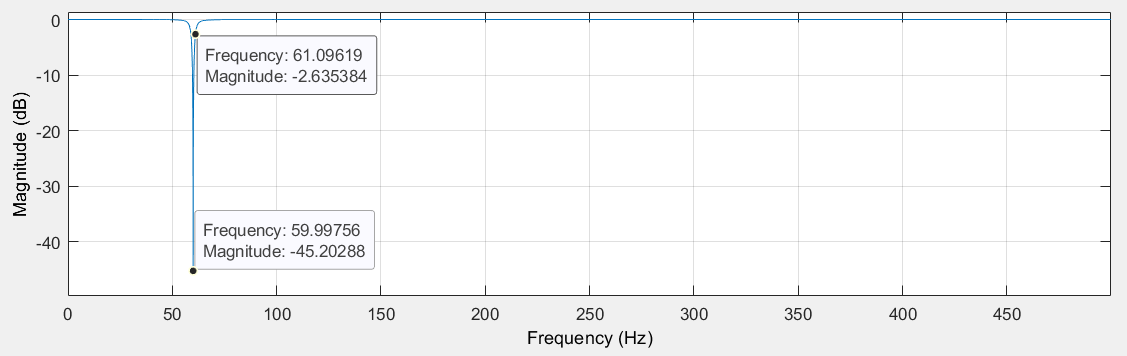
\includegraphics[width=1\linewidth]{figuras/preprocessing/notch_mag_response.png}
    }
    \caption{Magnitude response of the designed Notch filter. The frequency component at \qty{60}{Hz} is attenuated while having minimum effect on the EMG band.}
    \label{fig:notch_mag_response}
\end{figure}


However, the main drawback of this design the considerable variation in group delay around the power-line frequency. As shown in Figure \ref{fig:notch_group_delay_IIR}, the delay near cutoff frequencies reaches approximately 73-74 samples and remains high over the closer frequencies before decreasing.

This may impact the temporal structure of the signal components close to \qty{60}{Hz}. Even considering this effect, the IIR notch filter remains a realistic option for live implementation. In real world scenarios, the preferred solution would be to reduce the power-line interference at the signal acquisition stage instead of relying on digital signal processing. For this study, the anti-causal tool \textbf{\textit{filtfilt}} is used in order to prevent this major effect. 

\begin{figure}[H]
    \centering
    \makebox[\textwidth][c]{%
        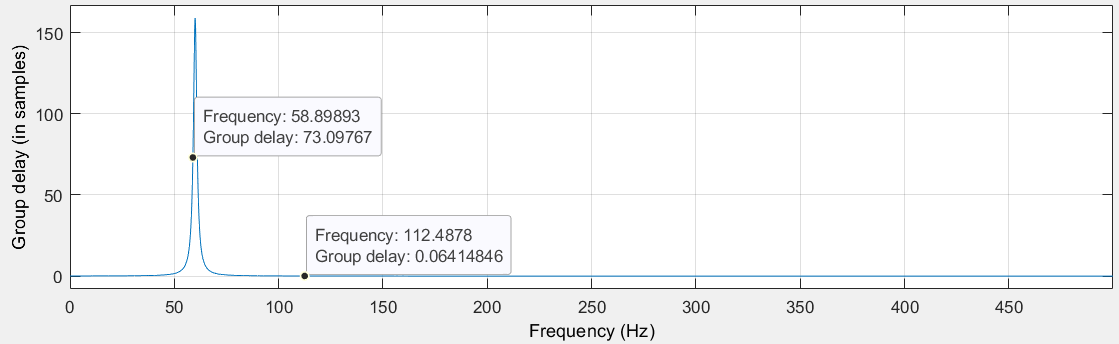
\includegraphics[width=1\linewidth]{figuras/preprocessing/notch_group_delay.png}%
    }
    \caption{Group delay of the designed notch filter. The cut-off frequencies experience a delay around \qty{73}{samples} which has considered when processing the signal. The best option in real world cases is to minimize power-line interference beforehand. }
    \label{fig:notch_group_delay_IIR}
\end{figure}
\subsubsection{EMG Frequency Range Filter}
Once the main power-line artifact has been attenuated, the next step is to retain only the frequency that contains relevant EMG information, while suppressing components outside this range. For this reason, a filter with the following characteristics is needed:

\begin{itemize}
    \item \textbf{Response type}: Bandpass
    \item \textbf{Design method}: Butterworth
    \item \textbf{Order}: 2
    \item \textbf{Cutt-off frequencies}: 
    \begin{itemize}
        \item f$_{HP} = \qty{20}{\hertz}\implies
\omega_{HP}
= 2\pi\frac{20}{1000}
= 0.04\pi \,\text{rad/sample}.$
        \item f$_{LP} = \qty{450}{\hertz}\implies
\omega_{LP}
= 2\pi\frac{450}{1000}
= 0.9\pi \,\text{rad/sample}.$
    \end{itemize}
\end{itemize}

The magnitude and phase responses of the designed IIR Butterworth filter are shown in Figure \ref{fig:mag_phase_response}.The magnitude response confirms that the filter preserves the mentioned EMG passband while attenuating the frequency components outside the range, showing a \qty{-3}{dB} attenuation at the cutting frequencies. Additionally, phase response shows a non-linear phase behavior which lead to different frequency components experiencing different phase shifts. 

\begin{figure}[H]
    \centering
    \makebox[\textwidth][c]{%
        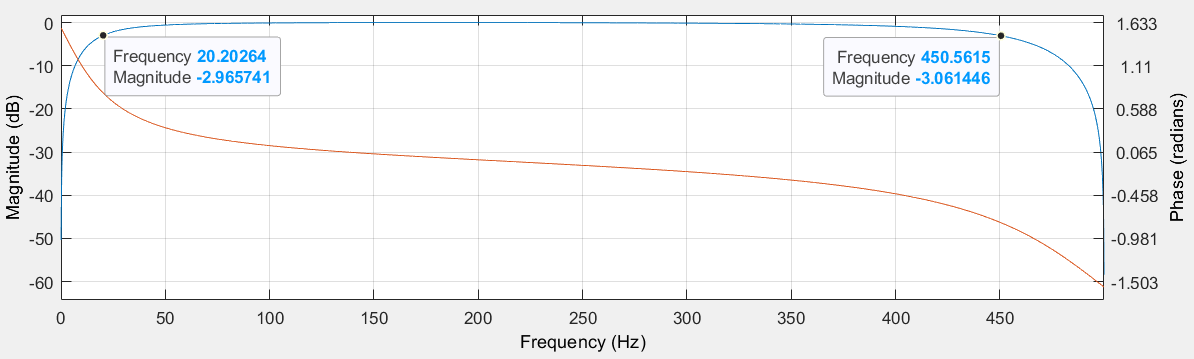
\includegraphics[width=1\linewidth]{figuras/preprocessing/mag_phase_response.png}%
    }
    \caption{Magnitude and phase response of the desgined bandpass filter.}
    \label{fig:mag_phase_response}
\end{figure}
To better understand this effect, Figure \ref{fig:group_delay_IIR} shows that the delay experienced at $f_H$ is around 4 samples, which at $f_s=$\qty{1}{kHz} is about \qty{4}{ms}. This delay decays over the 20-100 Hz band to approximately 0.21 ms and then increases across the \qtyrange{400}{450}{\hertz} band, reaching around \qty{1.68}{ms}. Although group delay often introduces frequency dependent temporal distortion, the magnitude of these delay variations is small compared to the duration of the signal and EMG activation. For this reason, the effect can be considered negligible for the posterior processing of the signal.
\begin{figure}[H]
    \centering
    \makebox[\textwidth][c]{%
        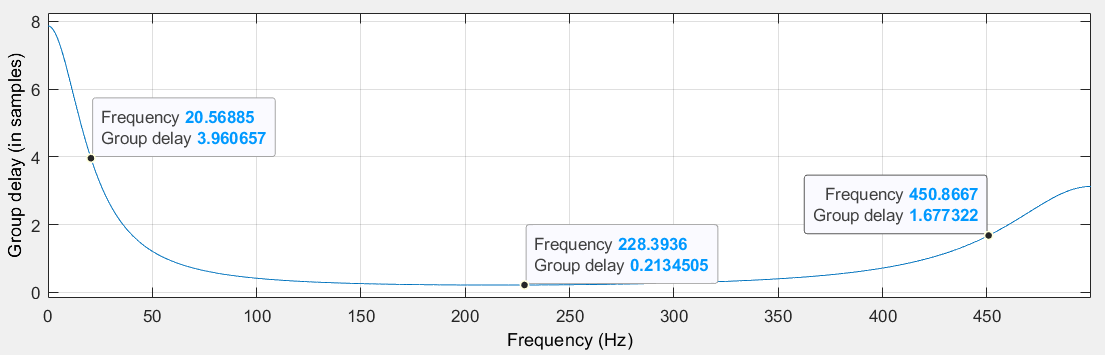
\includegraphics[width=1\linewidth]{figuras/preprocessing/group_delay.png}%
    }
    \caption{Group delay of the designed bandpass filter. Although a Bessel filter would provide a more constant delay, the Butterworth filter has a lower and nearly constant group delay within the EMG bandwidth.}
    \label{fig:group_delay_IIR}
\end{figure}

\subsection{Filtering results}
This section aims to evaluate the effect of the discussed filtering stage on the recorded EMG signals. To illustrate the filtering results, channel 1 is used as a representative example. The signal is analyzed both in the time domain and in the frequency domain before and after filtering. Although only one channel is shown, the same filtering procedure was applied to all channels.

\subsubsection{Time-Domain Analysis}

Given that EMG mainly conveys information about motor unit activation, this analysis should mainly focus on the RMS envelope of the signal in the time-domain. Figure \ref{fig:filtering_envelope_comparison} compares the RMS envelope of Channel 1 before and after filtering. The filtered signal presents a lower RMS amplitude due to the attenuation of undesired frequency components. However, the main EMG activation peaks still occur at approximately the same moments and the overall envelope shape is preserved. This suggests that the filtering stage reduces the artifacts without significantly altering the temporal activation pattern of the signal.

\begin{figure}[H]
    \centering
    \makebox[\textwidth][c]{%
        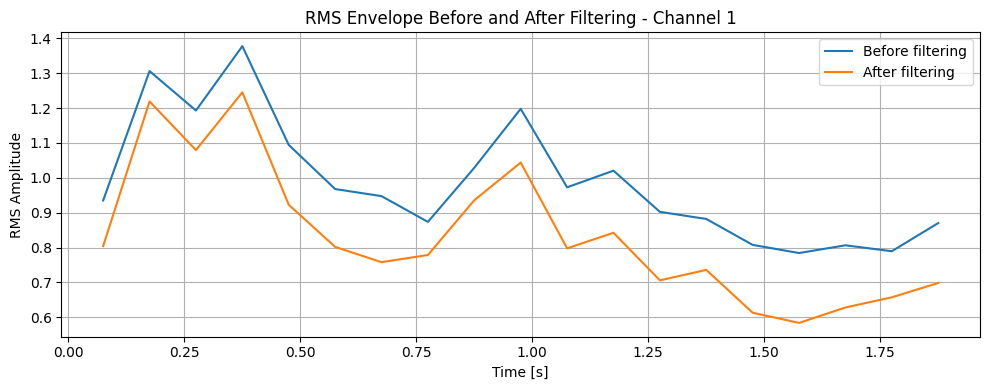
\includegraphics[width=1\linewidth]{figuras/preprocessing/filtering_envelop_comparison.png}%
    }
    \caption{Envelope comparison of filtered and unfiltered EMG channel 1 signal.}
    \label{fig:filtering_envelope_comparison}
\end{figure}


\subsubsection{Frequency-Domain Analysis}
The main goal of this analysis is to assess whether the designed filtering stage manages to remove undesired frequency components while preserving the original EMG frequency range. For this reason, the FFT magnitude spectrum and the power spectral density (PSD) of channel 1 were compared before and after filtering.
Figure \ref{fig:filtering_frequency_comparison} shows the frequency-domain comparison, which shows that the filtering stage attenuates the frequencies associated with the power-line interference as well as components outside the mentioned EMG band. The PSD of both unfiltered and filtered EMG signals, which confirms that the filtering stage manages to retain only the useful EMG frequencies.

\begin{figure}[H]
    \centering
    \makebox[\textwidth][c]{%
        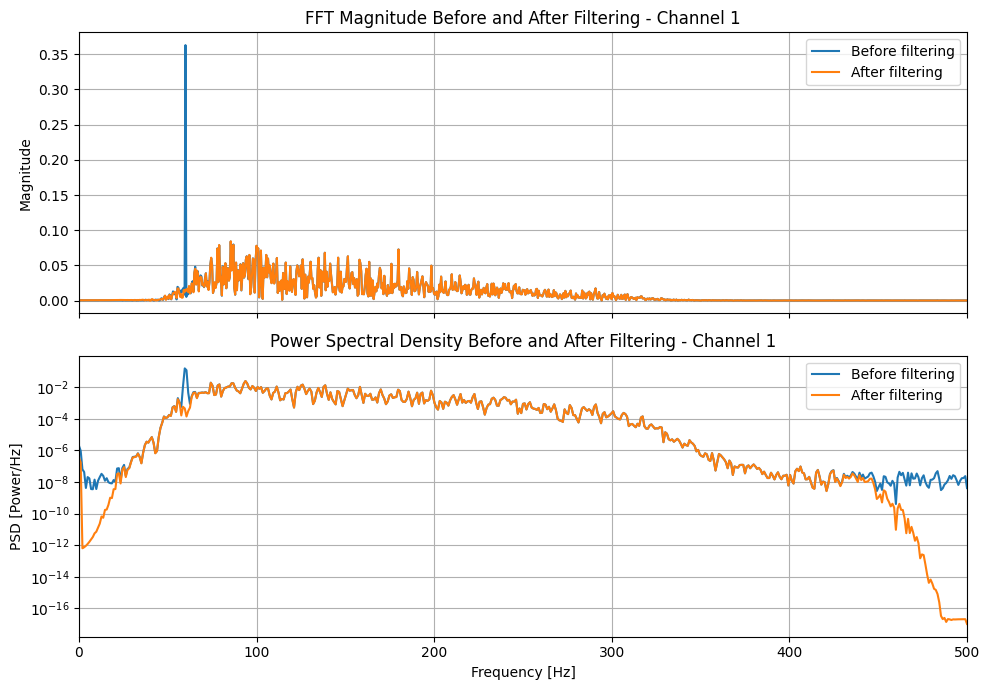
\includegraphics[width=1\linewidth]{figuras/preprocessing/filtering_frequency_comparison.png}%
    }
    \caption{Comparison of the FFT and PSD of Channel 1 before and after filtering. In regions where both signals have similar values, the filtered curve appears superimposed on the unfiltered curve. It is also worth to mention that the FFT magnitude plot is in natural scale while PSD is in logarithmic scale.}
    \label{fig:filtering_frequency_comparison}
\end{figure}

\section{Channel scaling}
The goal of this section is transform the recorded channels to a comparable numerical scale. This is especially important for multichannel EMG, since impedance, amplification or distance can make some channels dominate the covariance matrix even if they are not the most informative channels physiologically. Therefore, in this study, channel scaling is established as the combination of mean centering, outlier clipping and standardization as shown in Figure~\ref{fig:preprocessing_pipeline}. However, it is important to note that scaling is mainly used to improve the numerical behavior of the separation algorithms rather than to interpret the final source amplitudes directly.

\subsection{Mean centering}
\label{subsec:mean_centering}
Mean centering mainly intends to remove the DC component of each channel. Even though the EMG signal should ideally be zero mean after the filtering stage due to the bandpass filter, small offsets or motion artifacts may remain. This step is also required before covariance estimation and whitening. Considering the 32 channel EMG dataset, Equation \ref{eq:mean_centering} shows the mathematical procedure used for mean centering.

\begin{equation}
\mu_j = \frac{1}{N}\sum_{n=1}^{N} x_j[n],
\qquad
x_{c,j}[n] = x_j[n] - \mu_j  \quad \forall j=1,2,\dots,N 
\label{eq:mean_centering}
\end{equation}
\subsection{Outlier clipping}
The next step in the preprocessing is to apply outlier clipping to each observed EMG channel. The objective of this stage is limit isolated high-amplitude artifacts that could affect the RMS normalization and the covariance estimation used in later stages. This is especially relevant in the weak-source model considered in this work (section \ref{sec:weak_source_regime}) where the target source may be masked by a dominant component. To perform this operation, a robust median and median absolute deviation (MAD) criterion is used, since it is less sensitive to extreme values than mean and standard deviation thresholds\cite{hoaglin_volume_2013}.This choice is also motivated by the presence of transient artifacts and noise contamination in EMG recordings \cite{boyer_reducing_2023}.

For each observed channel \(c_j[n]\), the median and median absolute are computed as shown in Equation \ref{eq:mad_outlier}. Afterwards, the signal is then clipped to channel-dependent interval. Equation \ref{eq:outlier_clipping} depicts the mathematical expression for the clipping, where $k$ is a parameter that controls the clipping threshold in terms of MAD units.
\begin{equation}
m_j = \operatorname{median}\left(x_j[n]\right),
\quad
\operatorname{MAD}_j =
\operatorname{median}\left(\left|x_j[n]-m_j\right|\right)
\quad \forall j=1,2,\dots,N 
\label{eq:mad_outlier}
\end{equation}

\begin{equation}
x_{\text{clip},j}[n]
=
\min\left(
\max\left(x_j[n],\, m_j-k\operatorname{MAD}_j\right),
\, m_j+k\operatorname{MAD}_j
\right)
\quad \forall j=1,2,\dots,N 
\label{eq:outlier_clipping}
\end{equation} \\ \noindent
In this study, \(k=8\) was selected as a conservative threshold. Since clipping is a nonlinear operation, the value of \(k\) should be large enough to avoid attenuating actual EMG bursts, especially those related to the weak target component.
\subsection{RMS normalization}
After outlier clipping, each observed EMG channel is normalized by its RMS value. This step places all channels on a comparable energy scale before whitening and source separation.
\begin{equation}
z_j[n] =
\frac{x_{\text{clip},j}[n]}
{\operatorname{RMS}_j+\varepsilon}
\quad \forall j=1,2,\dots,N 
\label{eq:rms_scaling}
\end{equation}
where \(\varepsilon\) is small constant added to avoid indetermination problems when the RMS value is close to zero. Unlike the traditional z-score standardization, this operation does not substract the mean during the scaling stage, as the mean centering has already been applied previously in \ref{subsec:mean_centering}.

\section{Whitening}

Whitening is the last stage of the preprocessing pipeline. Its objective is to transform the scaled observations into a new representation whose components are uncorrelated and have unit variance. This step is especially useful before applying source separation algorithms as it removes second-order dependencies between channels and simplifies the conditioning of the problem.

Instead of describing the complete whitening derivation, this section only introduces its practical effect on the preprocessed EMG signals. Let $\mathbf{X_{scaled}}$ denote the centered channel-scaled observation matrix and $\mathbf{Z}$ the whitened data. The whitening transformation is expressed as a linear transformation applied to the centered observations:

\begin{equation}
    \mathbf{X}_w = \mathbf{P}\,\mathbf{X_{scaled}}
\end{equation}
where $\mathbf{P}$ represents the whitening transformation. The main idea of this operation is to obtain transformed observations whose covariance matrix is approximately equal to the identity matrix.

\begin{equation}
    \operatorname{Cov}(\mathbf{X}_w) \approx \mathbf{I}
\end{equation}
This means that the resulting components are decorrelated and normalized to unit variance. Figure~\ref{fig:whitening_effect} shows this effect in two-dimensional example. After whitening, the data are projected into a representation with approximately circular covariance, which simplifies the subsequent source separation stage.

\begin{figure}[H]
    \centering
    \makebox[\textwidth][c]{%
        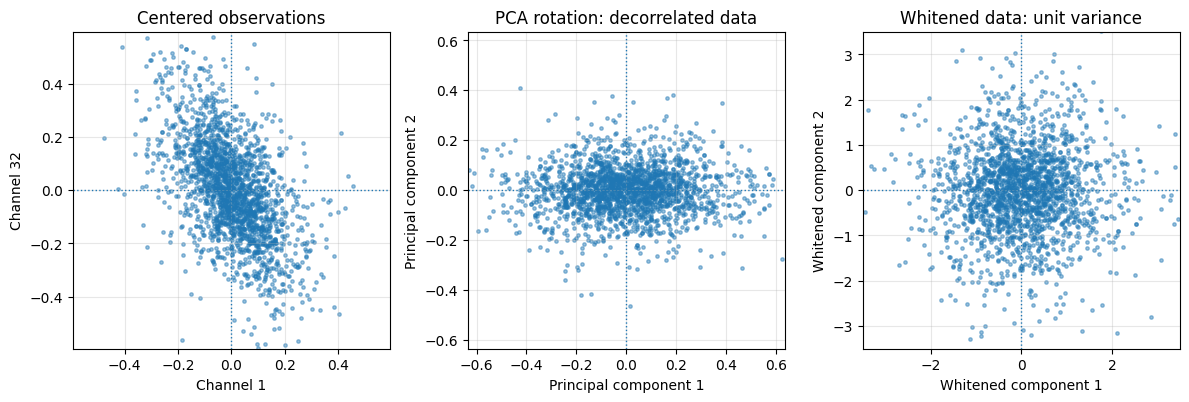
\includegraphics[width=1\linewidth]{figuras/preprocessing/whitening_effect.png}%
    }
    \caption{Visual whitening process for channels 1 and 32}
    \label{fig:whitening_effect}
\end{figure}

It is important to note that whitening does not perform source separation by itself. It only removes linear correlation and normalizes the variance of the observed components. Therefore, the resulting signals are decorrelated but not necessarily statistically independent. The remaining separation must be carried out by the subsequent algorithms, such as ICA, SOBI or constrained ICA. A more detailed geometric interpretation of whitening in the context of ICA is presented later in Section~\ref{sec:ica_derivation}.

\section{Considerations for real-time preprocessing}

Though the first filtering stage is designed to be implemented live, the channel scaling and signal decorrelation stages are inherently offline. Since the experiments of this thesis are mainly carried out with a prerecorded dataset, this may not result in a problem, but for real prosthetic implementation one of the following approaches should be considered:

\begin{itemize}
    \item \textbf{Fixed calibration strategy}
\end{itemize}
\noindent Preprocessing parameters are estimated once during an initial calibration stage:
    \[
        \mu_j,\quad \operatorname{MAD}_j,\quad \operatorname{RMS}_j,\quad \mathbf{P}
    \]
    where \(\mathbf{P}\) denotes the whitening matrix. These values are then kept fixed during online operation:
    \[
        \text{calibration data} \rightarrow \text{parameter estimation} \rightarrow \text{fixed online preprocessing}
    \]
    This approach is simple and stable, but assumes that the recording conditions do not change significantly after calibration.
\begin{itemize}
    \item \textbf{Sliding window adaptive strategy}
\end{itemize}
\noindent Preprocessing parameters are continuously updated using the most recent \(L\) samples:
    \[
        \mu_j[n],\quad \operatorname{MAD}_j[n],\quad \operatorname{RMS}_j[n],\quad \mathbf{P}[n]
    \]
    This allows the system to adapt over time:
    \[
        \text{recent window} \rightarrow \text{updated parameters} \rightarrow \text{adaptive online preprocessing}
    \]
    However, the main trade-off of this approach is:
    \[
        L \uparrow \Rightarrow \text{more accurate estimates, higher delay}
    \]
    \[
        L \downarrow \Rightarrow \text{lower delay, noisier estimates}
    \]
Given all these considerations, calibration-based preprocessing may be more stable and easier to implement if there is reliable calibration data. Otherwise, sliding windows approach is more adaptive but may introduce significant latency when preprocessing the EMG signals.
